\documentclass[border=10pt]{standalone}
\usepackage{pgfplots}
\pgfplotsset{compat=1.18}
\begin{document}
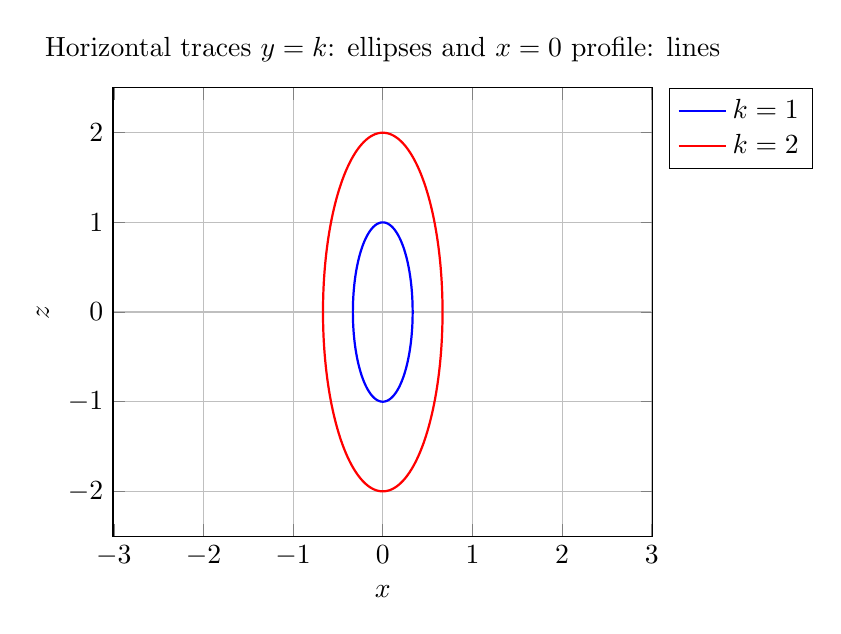
\begin{tikzpicture}
\begin{axis}[
    xlabel=$x$, ylabel=$z$,
    axis equal,
    title={Horizontal traces $y=k$: ellipses and $x=0$ profile: lines},
    xmin=-1.2, xmax=1.2, ymin=-2.5, ymax=2.5,
    grid=both,
    legend pos=outer north east,
]
\addplot[domain=0:360, samples=200, thick, blue] ({1/3*cos(x)}, {1*sin(x)});
\addplot[domain=0:360, samples=200, thick, red] ({2/3*cos(x)}, {2*sin(x)});
\legend{$k=1$, $k=2$}
\end{axis}
\end{tikzpicture}
\end{document}